\subsection{テキスト編集画面}
テキスト編集画面は観光スポットに対応するカードに表示する紹介文をユーザが編集する画面で、そのテキストは前述のカードリスト画面やマップ・詳細画面、後述の「振り返る」機能、印刷されるリーフレットに表記される。編集できる項目はタイトルと本文の2つである。この編集機能は、もともと観光スポットの説明が書かれているものを、ユーザがその場所で体験したことや起こったことに関するエピソードに置き換えることによって、思い出をより記憶深いものとして残す効果や、読み返したときの振り返りをより深いものにするという効果を期待して実装した。画面は図6.4のような構成になっていて、白い欄内の文字を書き替えて「保存する」ボタンをタップするとその結果が各画面に反映される。レイアウトは極力カードリストで表示されるものと同じようにして、ユーザが何を編集しているかが分かるよう工夫した。またタイトルと本文がそれぞれ編集可能であることを示すためにテキストエリアの背景色を白とし、この画面へ画面遷移した際に予めテキストエリアが選択され画面下にキーボードが表示される状態にした。ほかに、担当教員からの、ユーザが操作を誤ってもそれを取り消せる仕組みが必要との助言から「元に戻す」ボタンを配置した。これはユーザが誤って保存の操作をしてしまった場合の救済措置で、このボタンを押すことで文章を最初の状態に戻すことができる。また、ユーザの誤った操作を未然に防ぐための対策として、確認ダイアログを表示するようにした。テキストを変更して保存せずに前の画面に戻ろうとした場合や、もとに戻すボタンを押した際に、確認ダイアログで再度ユーザに確認を求めるステップを設けて誤った操作を減らす。
\newpage

\begin{figure}[htbp]
  \begin{center}
    \begin{tabular}{c}

      % 1
      \begin{minipage}{0.33\hsize}
        \begin{center}
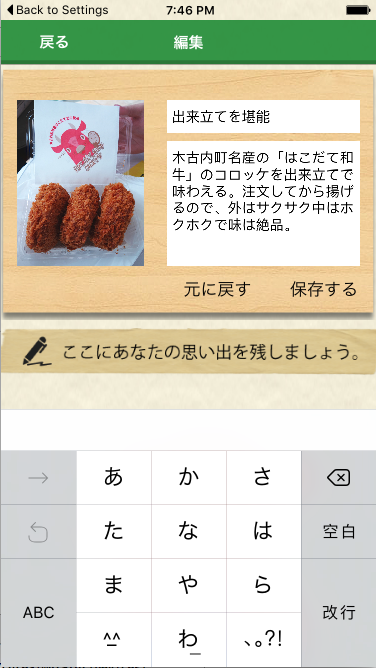
\includegraphics[width=4cm, bb=0 0 303 573]{kiko_edit.png}
        \end{center}
      \end{minipage}

    \end{tabular}
    \caption{テキスト編集画面}
    \label{fig:lena}
  \end{center}
\end{figure}

\bunseki{細川椋太}